% Created 2019-04-05 Fri 11:52
% Intended LaTeX compiler: pdflatex
\documentclass[11pt]{article}
\usepackage[utf8]{inputenc}
\usepackage[T1]{fontenc}
\usepackage{graphicx}
\usepackage{grffile}
\usepackage{longtable}
\usepackage{wrapfig}
\usepackage{rotating}
\usepackage[normalem]{ulem}
\usepackage{amsmath}
\usepackage{textcomp}
\usepackage{amssymb}
\usepackage{capt-of}
\usepackage{hyperref}
\usepackage{minted}
\usepackage[margin=2cm]{geometry}
\DeclareMathOperator{\sign}{sign}
\setlength{\parindent}{0cm}
\usepackage{pgfplots}
\pgfplotsset{compat=1.11}
\usetikzlibrary{arrows, decorations.markings}
\usetikzlibrary{3d}
\usetikzlibrary{shapes.geometric,decorations.fractals,shadows}
\date{\today}
\title{}
\hypersetup{
 pdfauthor={},
 pdftitle={},
 pdfkeywords={},
 pdfsubject={},
 pdfcreator={Emacs 26.1 (Org mode 9.2.2)}, 
 pdflang={English}}
\begin{document}


\section{Supervised learning}
\label{sec:orgb17e083}
Method where you train the program by feeding the learning algorithm with a mapping of
inputs to correct outputs.
\subsection{Regression}
\label{sec:org77518e2}
Regression is curve fitting: learn a continuous input \(\to\) output mapping from a set of
examples.
\subsection{Classification}
\label{sec:org7ba2ef9}
Outputs are discrete variables (category labels). Learn a decision boundary that
separates one class from the other. Generally, a confidence is also desired, i.e.,
how sure are we that the input belongs to the chosen category.
\subsection{Training set}
\label{sec:orgbc26ef5}
The training set is a set of \(m\) \((\vec{X},\, y)\) pairs, where:
\begin{align*}
  \vec{X} \in \mathbb{R}^d & \quad\text{models the input.} \\
  y \in \{0, 1\} & \quad\text{models the output.}
\end{align*}
\subsection{Error function}
\label{sec:orgf3f8320}
The error function for a model \(f: \vec{X} \mapsto y\) parameterized by \(\vec{W}\) applied to a
dataset \(\{ (\vec{X},\, y) \}\) of size \(m\) is:
\[
  \min_{\vec{W}} \left[ L(\vec{W}) = \sum^m_i{ \big(f_{\vec{W}}(\vec{X}_i) - y_i \big)^2 } \right]
\]
\subsection{Perceptron}
\label{sec:org40d0a26}
Perceptron is the trivial neural network. The model for a parameter \(\vec{W} = (\text{threshold},\,
   w_1,\, \hdots,\, w_d)\) and inputs of the form \((1,\, x_1,\, \hdots,\, x_d)\) is given by
\[
  f_{\vec{W}}(\vec{X}) = \sign(\vec{W} \vec{X})
\]
Where \(\sign\) is the activation function. \\
If \(x_i\) is evidence for approval, then \(w_i\) should be high. \\
If \(x_i\) is evidence for denial, then \(w_i\) should be low.
\subsubsection{Learning algorithm}
\label{sec:org29d1cd6}
The learning algorithm of the Perceptron is quite simple. The learning rate \(\in (0,\,
    1]\) is used to scale each step. the For a training set \(S = \{ \, (\vec{X}_1,\, y_1),\enspace (\vec{X}_2,\,
    y_2),\enspace \hdots \, \}\)
\begin{itemize}
\item Starting with random weights, then show each sample in sequence repetitively.
\item If the output is correct, do nothing.
\item If the produced output is negative, and the correct output is positive, increase the weights.
\item If the produced output is positive, and the correct output is negative, decrease the weights.
\item The amount to increase/decrease is given by the current sample scaled by the learning rate.
\end{itemize}
\subsection{Error}
\label{sec:orgb097b25}
The error function for a model \(f\) in a \textbf{training} sample is
\[ E_{\text{in}}(f) \]
This function is known and calculable.
\\[10pt]
The error function for a model \(f\) in a \textbf{test} sample is
\[ E_{\text{ou}t}(f) \]
This function is \textbf{not} known, and only \textbf{approachable}.
\\[10pt]
Given a model \(f\) in a set of \(M\) models, the bound for the probability of the error
deviation surpassing a given \(\epsilon\) is
\[
  \mathbb{P}\left(\big| E_{\text{in}}(f) - E_{\text{ou}t}(f) \big| > \big\epsilon\right) \leq 2Me^{-2N\big\epsilon^2}
\]
Notably, \(E_{\text{in}}(f)\) and \(E_{\text{out}}(f)\) deviates as \(f\) becomes complex.
\subsubsection{Empirical error minimization}
\label{sec:org658c23c}
During the learning algorithm, always conserve the weights that produce the lower error. \\
This has a disadvantage: It memorizes the training set.
\subsection{Ensemble learning}
\label{sec:org72a1d37}
Ensemble learning consists in combining several simple models to form a more complex
model.
\begin{description}
\item[{Bagging:}] Each model training with a different dataset
\item[{Boosting:}] Same dataset, but instrumented for each model to mitigate the weakness of
others
\end{description}
\subsection{Learning decision trees}
\label{sec:orgcea9bef}
Each layer in the tree consists of an attribute that splits the data into subsets that
are ideally disjoint. \\
The entropy of the subsets produced is a measure of how disjoint they are.
\\[5pt]
For a set containing \(p\) positive and \(n\) negatives, the entropy is
\[
  H\left(\frac{p}{p+n}, \frac{n}{p+n} \right) = - \frac{p}{p + n} \log\left( \frac{p}{p + n} \right) 
                                                - \frac{n}{p + n}\log\left( \frac{n}{p + n} \right)
\]
A given attribute \(A\), with \(k\) distinct values, divides the training set \(S\) into
subsets \(S_1, S_2, \hdots, S_k\). \\
The expected entropy remaining after applying \(A\) is
\[
  EH(A) = \sum_{i = 1}^{k} \left[ \frac{p_i + n_i}{p + n} \cdot H\left( \frac{p_i}{p_i + n_i}, \frac{n_i}{p_i + n_i} \right) \right]
\]
The information gain, i.e. the reduction in entropy for \(A\), is
\[
  I(A) = H\left( \frac{p}{p + n}, \frac{n}{p + n} \right) - EH(A)
\]
\subsection{Capacity}
\label{sec:orge899688}
The capacity is a measure of when the training error is a good approximation for the
test error.
\begin{figure}[H]
  \centering
  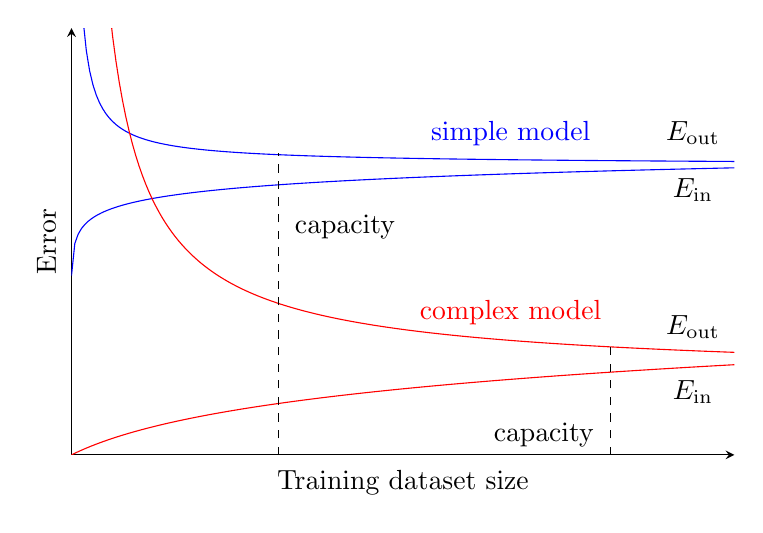
\begin{tikzpicture}
    \begin{axis}[
        axis lines = middle,
        xlabel near ticks,
        ylabel near ticks,
        xlabel     = {Training dataset size},
        ylabel     = {Error},
        xmin       = 0,
        ymin       = 0,
        ymax       = 15,
        height     = 7cm,
        width      = 10cm,
        xtick      = \empty,
        ytick      = \empty,
        black
      ]
      \addplot [
        samples=200,
        domain=0:8,
        blue
      ] {(ln(200*x + 1)/ln(7)) + 6.3};
      \addplot [
        samples=200,
        domain=0.1:8,
        blue
      ] {1/log2(x + 1) + 10};
      \addplot [
        samples=200,
        domain=0:8,
        red
      ] {log2(x + 1)};
      \addplot [
        samples=200,
        domain=0.1:8,
        red
      ] {1/log10(x/2.5 + 1) + 2};

      \draw [black, dashed] (axis cs: 6.5, 0) |- (axis cs: 6.5, 4);
      \draw [black, dashed] (axis cs: 2.5, 0) |- (axis cs: 2.5, 10.6);
      \node [black] at (7.5, 2.2) {$E_{\text{in}}$};
      \node [black] at (7.5, 4.5) {$E_{\text{out}}$};
      \node [black] at (7.5, 9.3) {$E_{\text{in}}$};
      \node [black] at (7.5, 11.3) {$E_{\text{out}}$};
      \node [blue] at (5.3, 11.3) {simple model};
      \node [red] at (5.3, 5) {complex model};
      \node [black] at (3.3, 8) {capacity};
      \node [black] at (5.7, 0.7) {capacity};

    \end{axis}
  \end{tikzpicture}
\end{figure}
\subsection{Bias and variance}
\label{sec:orgd904fba}
\textbf{Bias} is the error due to the fact that the set of functions does not contain the
target function.
\\[5pt]
\textbf{Variance} is the error due to the fact that if we had been using another training set
drawn from the same distribution, we would have obtained another function.
\\[5pt]
\textbf{Regularization} is a method for minimizing the training error, as long as it is still a
good approximation for the test error, trading-off accuracy for simplicity.
\subsection{Single layer neural networks}
\label{sec:orga1371e6}
Using the sigmoid as the activation function, and the squared-error loss function:
\[
  L(\vec{W}) = \frac{1}{2} \sum_i^m \left( \sigma\left(\vec{W} \vec{X}_i\right) - y_i \right)^2
\]
To find in which direction the weights minimizes \(L\), the gradient is used:
\[
  \nabla L(\vec{W}) = \sum_i^m \Delta \cdot \Psi
\]
Where the delta rule is
\[
  \Delta = \vec{X}_i \cdot \left( \sigma\left(\vec{W}\vec{X}_i\right) - y_i \right)
\]
And the slope of ligistic is
\[
  \Psi = \sigma\left(\vec{W}\vec{X}_i\right) \cdot \left(1 - \sigma\left(\vec{W}\vec{X}_i\right)\right)
\]
\newpage
\subsubsection{Gradient descent algorithm}
\label{sec:org269215e}
The learning rate \(r \in (0,\, 1]\) is used to scale each step.
\begin{enumerate}
\item Starting with random weights.
\item Compute \(\nabla L(\vec{W})\).
\item \(\vec{W} \leftarrow \vec{W} - r \cdot \nabla L(\vec{W}) = \vec{W} - r \cdot \sum\limits_i^m \Delta \Psi\)
\item Repeat steps 2 and 3 until \(\vec{W}\) doesn't change anymore \((10^{-5})\).
\end{enumerate}
After each iteration, \(L(\vec{W})\) should be checked:
\begin{enumerate}
\item If \(L(\vec{W})\) is converging, the learning rate is correct.
\item If \(L(\vec{W})\) is diverging, the learning rate is too large.
\item If \(L(\vec{W})\) is converging slowly, the learning rate too small.
\end{enumerate}
Also, the algorithm needs feature scaling
\[
  x'_i = \frac{x_i - \min(\vec{X})}{\max(\vec{X}) - \min(\vec{X})}
\]
\subsubsection{Stochastic gradient descent}
\label{sec:org1f9467f}
Instead of inspecting the whole dataset to detect the direction which minimize \(L\), a
single random sample is picked on each step.
\begin{enumerate}
\item Randomly shuffle the training set.
\item Starting with random weights.
\item For each sample \((\vec{X_i}, y_i)\): \(\>\vec{W} \leftarrow \vec{W} - r \cdot \Delta \Psi\)
\item Repeat step 3 until \(\vec{W}\) doesn't change anymore \((10^{-5})\).
\end{enumerate}
Convergence is not so obvious. After each bulk of iterations, e.g. 1000, check \(L(\vec{W})\):
\begin{enumerate}
\item If \(L(\vec{W})\) is converging, the learning rate is correct.
\item If \(L(\vec{W})\) is diverging, the learning rate is too large.
\item If \(L(\vec{W})\) is converging slowly, the learning rate too small.
\end{enumerate}
\subsubsection{Mini batches}
\label{sec:org49a42f0}
While GD uses all samples in each iteration, SGD uses only one. A possible middle
ground is to use a mini batch of samples in each iteration.
\[
  \vec{W} \leftarrow \vec{W} - r \cdot \frac{1}{b} \sum\limits_i^b \Delta \Psi
\]
Where \(b\) is the batch size, tipically \(10\).
\subsubsection{Regularization}
\label{sec:org34bfd39}
To prevent large weights, the norm of the weights is added to the loss function:
\[
  L(\vec{W}) = |\vec{W}| + \frac{1}{2} \sum_i^m \left( \sigma\left(\vec{W} \vec{X}_i\right) - y_i \right)^2
\]
\subsubsection{Early stopping (cross validation)}
\label{sec:orga9368c6}
Other way to improve is to prevent overfitting:
\begin{enumerate}
\item Separate the data into training and validation sets.
\item Minimize \(L(\vec{W})\) on the training set, stopping when \(L(\vec{W})\) on the validation set
stops improving.
\end{enumerate}
\section{Reinforcement learning}
\label{sec:orgcd35180}
Method where you train the program by rewarding the learning algorithm positively or
negatively according to the produced results. This method is similar to how we teach
animals.
\section{Unsupervised learning}
\label{sec:orgae4d9a1}
Given only inputs as training, find a pattern: discover clusters, manifolds, embedding.
\end{document}
